%appendix A
%SOURCE KEY SINK MODEL

\section{Process: Source Property}

\subsection{Visual}
\begin{figure}[ht]
    \centering
    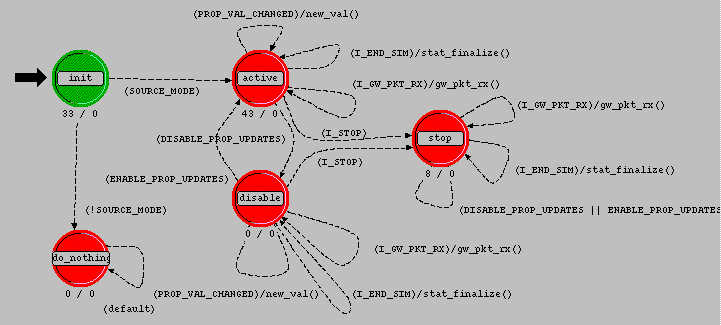
\includegraphics[width=.7\textwidth]{images/p_source_property}
    \caption{Source property process model}
    \label{fig:appendix-a}
\end{figure}

\subsection{Local variables}
\begin{figure}[ht]
    \centering
    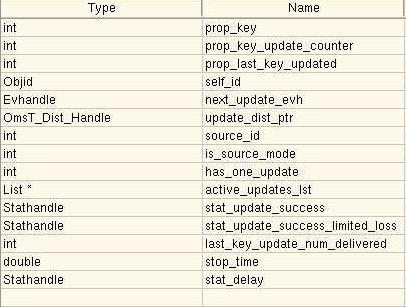
\includegraphics[width=.7\textwidth]{images/state_variable_source_property}
    \caption{State variables of source property process}
    \label{fig:appendix-a_sv}
\end{figure}

\subsection{Header Block}
%_____________________________________HEADER______________________________________
{\tiny
\begin{verbatim}
#include	<oms_dist_support.h>

//Interrupt Codes (codes have no meaning and are random)
#define IC_PROP_VAL_CHANGED 		39
#define IC_UPDATES_DISABLE	 		83
#define IC_UPDATES_ENABLE			84
#define IC_STOP					21
#define IC_GW_PKT_RX				99
#define SOURCE_MODE		(is_source_mode)

//Interrupts 
#define PROP_VAL_CHANGED	(op_intrpt_type() == OPC_INTRPT_SELF && op_intrpt_code() == IC_PROP_VAL_CHANGED)
#define DISABLE_PROP_UPDATES	(op_intrpt_type() == OPC_INTRPT_REMOTE && op_intrpt_code() == IC_UPDATES_DISABLE)
#define ENABLE_PROP_UPDATES	(op_intrpt_type() == OPC_INTRPT_REMOTE && op_intrpt_code() == IC_UPDATES_ENABLE)
#define I_GW_PKT_RX	(op_intrpt_type() == OPC_INTRPT_REMOTE && op_intrpt_code() == IC_GW_PKT_RX)
#define I_END_SIM	(op_intrpt_type() == OPC_INTRPT_ENDSIM)
#define I_STOP	(op_intrpt_type() == OPC_INTRPT_SELF && op_intrpt_code() == IC_STOP)

typedef struct
{
	int update_counter_number;
	int pkts_alive;
	int has_one_store;
	int gateway_rx;
	double generated_timestamp;
	int mark_for_delete;
	int discard_reason;
} active_update_tacker;

void new_val(void);
void schedule_update(void);
void gw_pkt_rx(void);
void stat_finalize(void);
\end{verbatim}
}

\subsection{Function Block}
%______________________________FUNCTION__________________________________
{\tiny
\begin{verbatim}

void new_val(void)
{
	FIN (new_val ());
	prop_key_update_counter++;
	schedule_update();
	FOUT
}
void schedule_update(void)
{
	double next_update_time;	
	FIN(schedule_update());
	next_update_time = oms_dist_outcome (update_dist_ptr);

	if (next_update_time <0)
	{
		next_update_time = 0;
	}

	next_update_evh      = op_intrpt_schedule_self (op_sim_time () + next_update_time, IC_PROP_VAL_CHANGED);
	FOUT;
}
void gw_pkt_rx()
{
	Ici *iciptr;
	int sourceid;
	int key_update_number;
	int action;
	int discard_reason;
	int tracker_index;
	double generated_timestamp;
	active_update_tacker *pTracker;
	char msg[255];
	int i;

	FIN(gw_pkt_rx());
	iciptr = op_intrpt_ici ();
	
	if(iciptr == OPC_NIL)
	{
		op_sim_end("Null ICI", "", "", "");
	}
	op_ici_attr_get (iciptr, "source_id", &sourceid);
	op_ici_attr_get (iciptr, "key_update_number", &key_update_number);
	op_ici_attr_get (iciptr, "action", &action);
	op_ici_attr_get (iciptr, "discard_reason", &discard_reason);
	op_ici_attr_get (iciptr, "generated_timestamp", &generated_timestamp);

	//Basic field checks 
	if(sourceid != source_id)
	{
		op_sim_end("Bad source id for ICI", "", "", "");
	}
	else if(key_update_number > prop_key_update_counter || key_update_number <= 0)
	{
		op_sim_end("Bad key_update_number for ICI", "", "", "");
	}	
	//Find the tracker
	pTracker = OPC_NIL;
	for(tracker_index = 0; tracker_index < op_prg_list_size(active_updates_lst); tracker_index++)
	{
		active_update_tacker *pTrackerTemp;
		pTrackerTemp = (active_update_tacker *)op_prg_list_access(active_updates_lst, tracker_index);
		
		if(pTrackerTemp->update_counter_number == key_update_number)
		{
			pTracker = pTrackerTemp;
			break;
		}
	}
	if(pTracker == OPC_NIL)
	{
		int i;
		char msg1[255];
		char msg2[255];
		char msg3[255];
		printf("Current list state\n");
		
		for(i = 0; i < op_prg_list_size(active_updates_lst); i++)
		{
			active_update_tacker *pTrackerTemp;
			pTrackerTemp = (active_update_tacker *)op_prg_list_access(active_updates_lst, i);	
			sprintf(msg1, "update_counter_number=%d\n", pTrackerTemp->update_counter_number);
			printf(msg1);
		}
		sprintf(msg1, "Tracker index=%d, List size=%d", tracker_index, op_prg_list_size(active_updates_lst));
		sprintf(msg2, "key_update_number=%d, prop_key_update_counter=%d", key_update_number, prop_key_update_counter);
		sprintf(msg3, "Action=%d", action);	
		op_sim_end("Could not find tracker", msg1, msg2, msg3);
	}
	if(action == 1)
	{
		//Gateway received packet
		if(pTracker->gateway_rx)
		{
			op_sim_end("Two gateway rx interrupts", "", "", "");
		}
		else if(pTracker->pkts_alive <= 0)
		{
			op_sim_end("pkts_alive problem", "", "", "");
		}
		pTracker->gateway_rx = 1;	
		op_stat_write(stat_delay, op_sim_time() - generated_timestamp);
		op_stat_write(stat_update_success, 1.0);
		op_stat_write(stat_update_success_limited_loss, 1.0);
		
		if(last_key_update_num_delivered >= key_update_number)
		{
			op_sim_end("Problem with gateway", "", "", "");
		}
		last_key_update_num_delivered = key_update_number;
	}
	else if (action == 2)
	{
		//Store	
		if(pTracker->pkts_alive < 0)
		{
			op_sim_end("Thats strange...", "", "", "");
		}	
		pTracker->pkts_alive++;
		pTracker->has_one_store = 1;
	}
	else if (action == 3)
	{
		//Discard
		pTracker->pkts_alive--;
		pTracker->discard_reason = discard_reason;
	}
	else
	{
		op_sim_end("Bad action", "", "", "");
	}
	has_one_update = 1;
	
	for(i = 0; i < op_prg_list_size(active_updates_lst); i++)
	{
		pTracker = (active_update_tacker *)op_prg_list_access(active_updates_lst, i);
	
		if(pTracker->pkts_alive <= 0)
		{
			pTracker->mark_for_delete--;
		}
		if(pTracker->mark_for_delete <= 0)
		{
			active_update_tacker *pTrackerTemp;
			
			if(pTracker->pkts_alive < 0 &&  pTracker->has_one_store)
			{
				op_sim_end("Thats strange...", "2", "", "");
			}	
			if(pTracker->gateway_rx == 0)
			{
				//Nothing left - update has been lost
				op_stat_write(stat_update_success, 0.0);
			
				if(pTracker->discard_reason == 1)
				{
					//Update
				}
				else if(pTracker->discard_reason == 2)
				{
					//Mem full
					if(pTracker->update_counter_number > last_key_update_num_delivered)
					{
						op_stat_write(stat_update_success_limited_loss, 0.0);
					}
				}
				else
				{
					op_sim_end("Bad discard reason", "", "", "");
				}
			}	
			pTrackerTemp = (active_update_tacker *)op_prg_list_remove(active_updates_lst, i);
			
			if(pTrackerTemp != pTracker)
			{
				op_sim_end("AHA,not another error!", "", "", "");
			}
			op_prg_mem_free(pTracker);
		}
	}
	op_ici_destroy(iciptr);
	FOUT;
}
void stat_finalize()
{
	Stathandle oneup;
	int i;

	FIN(stat_finalize());	
	oneup = op_stat_reg("One Update",OPC_STAT_INDEX_NONE, OPC_STAT_GLOBAL);	
	op_stat_write(oneup, has_one_update);
	
	for(i = 0; i < op_prg_list_size(active_updates_lst); i++)
	{
		active_update_tacker *pTracker;
		pTracker = (active_update_tacker *)op_prg_list_access(active_updates_lst, i);
		
		if(pTracker->gateway_rx == 0)
		{
			//Receiving should already have been taken care of
			op_stat_write(stat_update_success, 0.0);
			
			if(pTracker->update_counter_number > last_key_update_num_delivered)
			{
				op_stat_write(stat_update_success_limited_loss, 0.0);
			}
		}
		
		if(pTracker->update_counter_number == prop_last_key_updated)
		{
			if(pTracker->gateway_rx == 0)
			{
				op_stat_write(stat_delay, op_sim_time() - pTracker->generated_timestamp);
			}
		}
	}
	FOUT;
}
\end{verbatim}
}
\subsection{Init State}
%______________________________________Init_____________________________________________________________
{\tiny
\begin{verbatim}
char msg[100];
char updatedist_str [128];
self_id = op_id_self();
op_ima_obj_attr_get (self_id, "Source ID", &source_id);
op_ima_obj_attr_get (self_id, "Property Key", &prop_key);
op_ima_obj_attr_get (self_id, "Property Update Interval", updatedist_str);
op_ima_obj_attr_get (self_id, "Stop Time", &stop_time);
op_ima_obj_attr_get (self_id, "Enable Properties", &is_source_mode);
active_updates_lst = op_prg_list_create();
has_one_update = 0;
prop_key_update_counter = 0;
prop_last_key_updated = 0; //So it gets updated right away
update_dist_ptr = oms_dist_load_from_string (updatedist_str);
stat_delay = op_stat_reg("Delay",OPC_STAT_INDEX_NONE, OPC_STAT_GLOBAL);
stat_update_success = op_stat_reg("Update Success",OPC_STAT_INDEX_NONE, OPC_STAT_GLOBAL);
stat_update_success_limited_loss = op_stat_reg("Update Success - Losses by buffer full",OPC_STAT_INDEX_NONE, OPC_STAT_GLOBAL);

if(is_source_mode)
{
	schedule_update();	
	if(stop_time > 0)
	{
		op_intrpt_schedule_self (op_sim_time() + stop_time, IC_STOP);
	}
}
\end{verbatim}
}

\subsection{Active State}
%______________________________________Active_____________________________________________________________
{\tiny
\begin{verbatim}
Packet *pPkt;
if(prop_key_update_counter != prop_last_key_updated)
{
	active_update_tacker *pTracker;
	int i;
	
	//Error check
	for(i = 0; i < op_prg_list_size(active_updates_lst); i++)
	{
		//Might be able to just check the tail instead
	
		pTracker = (active_update_tacker *)op_prg_list_access(active_updates_lst, i);
		if(pTracker->update_counter_number == prop_last_key_updated)
		{
			if(pTracker->has_one_store == 0)
			{
				op_sim_end("Did not receive store interrupt", "", "", "");
			}
		}
	}
	prop_last_key_updated = prop_key_update_counter;
	pPkt = op_pk_create_fmt("keyupdate");
	op_pk_nfd_set_int32(pPkt, "source_id", source_id);		
	op_pk_nfd_set_int32(pPkt, "key", prop_key);	
	op_pk_nfd_set_int32(pPkt, "key_update_number", prop_key_update_counter);
	op_pk_nfd_set_dbl(pPkt, "generated_timestamp", op_sim_time());
	op_pk_nfd_set_objid(pPkt, "source_prop_objid", self_id);
	pTracker = (active_update_tacker *) op_prg_mem_alloc (sizeof (active_update_tacker));
	pTracker->update_counter_number = prop_key_update_counter;
	pTracker->pkts_alive = 0;
	pTracker->has_one_store = 0;
	pTracker->gateway_rx = 0;
	pTracker->generated_timestamp = op_sim_time();
	pTracker->mark_for_delete = 3;
	op_prg_list_insert(active_updates_lst, pTracker, OPC_LISTPOS_TAIL);	
	op_pk_send(pPkt, 0); //Output stream
}
\end{verbatim}
}

\subsection{Stop State}
%_____________________________________Stop_____________________________________________________________
{\tiny
\begin{verbatim}
char msg_str[255];
if (op_ev_valid (next_update_evh) == OPC_TRUE)
{
	sprintf(msg_str, "[%d] Stopping property updates @ %d\n", source_id, op_sim_time());
	printf(msg_str);
	op_ev_cancel (next_update_evh);
}
\end{verbatim}
}